\documentclass[../main/main.tex]{subfiles}
\graphicspath{{./figures/}}

\makeatletter
\renewcommand{\@chapapp}{Travaux pratiques -- TP}
\makeatother

% \toggletrue{student}
\toggletrue{corrige}
% \renewcommand{\mycol}{black}
% \renewcommand{\mycol}{gray}

\hfuzz=5.003pt

\begin{document}
\setcounter{chapter}{28}

\settype{enon}
\settype{solu_prof}
\settype{solu_stud}

\chapter{\cswitch{%
	  Correction du TP
  }{%
	  Observation numérique de cristaux
  }%
 }

\enonce{%
	\begin{tcn}*(exem)<ctc>"how"'t'{Capacités exigibles}
		\begin{itemize}
			\item Utiliser un logiciel ou des modèles cristallins pour visualiser des
			      mailles et des sites interstitiels et pour déterminer des paramètres
			      géométriques.
		\end{itemize}
	\end{tcn}
	\vspace{-10pt}
	\section{Objectifs}
	\begin{itemize}
		\item Visualiser à l'aide d'outils numériques des structures cristallines
		      (parfaites).
		\item Se familiariser avec l'observation des différents types de sites et de
		      structures.
		\item Bien comprendre les règles de construction de cristaux ioniques.
	\end{itemize}

	\section{S'approprier}

	Lancer le logiciel en ligne \texttt{minusc}~: \url{https://libmol.org/minusc/}.
	\begin{itemize}
		\item L'onglet \texttt{Commandes} permet de modifier l'affichage de la maille.
		\item L'onglet \texttt{Fichier} permet de changer de structure cristalline.
		\item L'onglet \texttt{Formule} permet d'afficer seulement certains atomes de
		      la maille. Pour revenir à la maille complète, on peut cliquer sur
		      \texttt{désactiver le mode formule} en bas à gauche.
	\end{itemize}
	\bigbreak
	\noindent
	\begin{minipage}[t]{.5\linewidth}
		\begin{itemize}
			\item Les paramètres de maille (distance $a,b,c$ et angles $\alpha, \beta,
				      \gamma$) sont affichés en haut à gauche de l'écran. Les distances
			      sont données en Angström~: $\SI{1}{\angstrom} = \SI{e-10}{m}$.

			\item La distance entre deux motifs peut être mesurée en double-cliquant
			      sur un motif, puis en pointant le second.
		\end{itemize}
	\end{minipage}
	\hfill
	\noindent
	\begin{minipage}[t]{.5\linewidth}
		~
		\vspace{-20pt}
		\begin{center}
			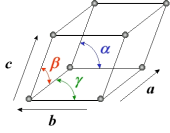
\includegraphics[scale=1]{pmaille}
			\captionof{figure}{Définition paramètres de maille.}
			\label{fig:pmaille}
		\end{center}
	\end{minipage}
	\begin{itemize}
		\item Plusieurs mailles peuvent être affichées en changeant les valeurs de
		      $a,b,c$ en bas à droite~: $a=2$ signifie «~afficher 2 mailles selon
		      l'axe de $a$~».
	\end{itemize}
}%

\section{Réaliser}
\label{sec:real}
\subsection{Étude d'une structure métallique~: argent}
\label{ssec:ag}
\enonce{%
	Dans \texttt{Fichier}, rechercher le cristal Argent.
}%
\resetQ
\setlist[blocQR,1]{leftmargin=10pt, label=\sqenumi}
\QR{%
	Quelle est la configuration cristallographique de l'argent~?
}{%
	solu
}%
\QR{%
	Quelle est la population de la maille~? La coordinence des atomes
	d'argent~?
}{%
	solu
}%
\QR{%
	Dans \texttt{Afficher atomes}, choisir \texttt{sphères}. Observer la
	tangence des atomes. Sachant que le rayon métallique des atomes d'argent
	vaut $r = \SI{144}{pm}$, en déduire la valeur du paramètre de maille
	théorique $a$. Le comparer au paramètre de maille réel.
}{%
	solu
}%
\QR{%
	Repérer et représenter les sites interstitiels tétraédriques et
	octaédriques.
}{%
	solu
}%

\subsection{Étude de plusieurs structures ioniques \hfill \small D'après
	Mines-Pont}
\label{ssec:ions}
% Les règles de construction des cristaux ioniques sont souvent énoncées comme
% suit (avec pour principe que les anions sont plus gros que les cations)~:
% \begin{itemize}[label=$\diamond$, leftmargin=10pt]
%   \litem{Règle 1}~: le cristal est électriquement neutre.
%   \litem{Règles 2}~:
%   \begin{itemize}[label=$\triangleright$, leftmargin=20pt]
%     \litem{2a}~: les anions de rayon $r_{-}$ forment un réseau (dit réseau-hôte) dans
%     lequel les cations de rayon $r_{+}$ occupent les sites interstitiels~;
%     \litem{2b}~: les cations sont entourés d'anions, la distance cation-anion la
%     plus courte est déterminée par la somme des rayons ioniques (les ions de
%     signes opposés sont considérés comme des sphères dures en contact)~;
%     \litem{2c}~: chaque cation est entouré du plus grand nombre d'anions pouvant
%     géométriquement se trouver à son contact (donc la coordinence doit être
%     maximale).
%   \end{itemize}
%   \litem{Règle 3}~: dans une structure donnée, le rapport de la charge sur la
%   coordinence est le même en valeur absolue pour le cation et pour l'anion.
% \end{itemize}
\QR{%
	Sachant que les anions sont plus gros que les cations, indiquer une
	première inégalité du rapport $\frac{r_{+}}{r_{-}}$, sous la forme
	$\frac{r_{+}}{r_{-}} < x$.
}{%
	solu
}%

\subsubsection{Étude de la structure type \ce{CsCl}}
\label{sssec:cscl}
\enonce{%
	Dans \texttt{Fichier}, recherchez le cristal \ce{CsCl} en écrivant
	\texttt{chlorure de césium}.
	\begin{tcb}(data)<lft>'l'{Données}
		$r_{+} = \SI{169}{pm}$ et $r_{-} = \SI{181}{pm}$.
	\end{tcb}
}%
\QR{%
	Où se situe \ce{Cs^+}~? Quelle est sa coordinence~? (On pourra choisir
	d'afficher 2 mailles par 2 mailles).
}{%
	solu
}%

\QR{%
	En visualisation 1 maille par 1 maille, où se situe
	\ce{Cl-}~? Quelle est sa coordinence~?
}{%
	solu
}%

\QR{%
	Comment avait-on décrit le chlorure de césium dans le cours~? Quels
	étaient les sites occupés par \ce{Cl-} et \ce{Cs+}~? Montrer que ces deux
	descriptions sont équivalentes.
}{%
	solu
}%

\QR{%
	Dans \texttt{afficher atomes}, choisir \texttt{sphères}. Observer la
	tangence des anions et des cations. Sachant que $r_{+} = \SI{169}{pm}$ et
	$r_{-} = \SI{181}{pm}$, déterminer le paramètre théorique $a_{\rm th}$ de la
	maille.
}{%
	solu
}%

\QR{%
	Le comparer au paramètre $a_{\rm exp}$. En déduire l'écart relatif sur $a$
	avec le modèle de sphères dures. Est-ce qu'il justifie l'emploi du modèle
	utilisé~?
}{%
	solu
}%

\QR{%
	Sans le logiciel~: d'après les règles de stabilité d'une structure
	ionique, déterminer une deuxième limite au rapport $\frac{r_{+}}{r_{-}}$
	pour cette structure.
}{%
	solu
}%

\QR{%
	Donner donc les 2 inégalités sur $\frac{r_{+}}{r_{-}}$ (cf.\ question
	\fbox{5}). Est-ce vérifié pour ce cristal~?
}{%
	solu
}%

\subsubsection{Étude de la structure type \ce{NaCl}}
\label{sssec:nacl}
\enonce{%
	Dans \texttt{Fichier}, recherchez le cristal \ce{NaCl} en écrivant \texttt{halite}.
	\begin{tcb}(data)<lft>'l'{Données}
		$r_{+} = \SI{95}{pm}$ et $r_{-} = \SI{181}{pm}$.
	\end{tcb}
	\begin{center}
		\begin{framed}
			\large
			Mêmes questions de 13 à 19 que pour \ce{CsCl}.
		\end{framed}
	\end{center}
}%

% \begin{enumerate}[label=\sqenumi, start=13]
%   \item Quel type de site occupe \ce{Na^+}~? Quelle est la coordinence de
%     \ce{Na+}~?
%   \item Quel type de site occupe \ce{Cl-}~? Quelle est sa coordinence~?
%   \item Comment avait-on décrit le chlorure de sodium dans le cours~? Quels
%     étaient les sites occupés par \ce{Cl-} et \ce{Na+}~? Montrer que ces deux
%     descriptions sont équivalentes, respectant donc la règle 2a.
%   \item Dans \texttt{afficher atomes}, choisir \texttt{sphères}. Observer la
%     tangence des anions et des cations. Sachant que $r_{+} = \SI{95}{pm}$ et
%     $r_{-} = \SI{181}{pm}$, déterminer le paramètre théorique $a_{\rm th}$ de la
%     maille.
%   \item Le comparer au paramètre $a_{\rm exp}$. En déduire l'erreur relative
%     commise sur $a$ avec le modèle de sphères dures. Est-ce qu'il justifie
%     l'emploi du modèle utilisé~?
%   \item Sans le logiciel~: d'après la règle 2b d'une part et du non-contact
%     entre mêmes charges, déterminer une deuxième limite au rapport
%     $\frac{r_{+}}{r_{-}}$.
%   \item Donner donc l'inégalité complète sur $\frac{r_{+}}{r_{-}}$. Est-ce
%     vérifié pour cette structure~?
% \end{enumerate}

\subsubsection{Étude de la structure type \ce{ZnS}}
\label{sssec:zns}
\enonce{%
	Dans \texttt{Fichier}, recherchez le cristal \ce{ZnS} en écrivant \texttt{ZnS}.
	\begin{tcb}(data)<lft>'l'{Données}
		$r_{+} = \SI{74}{pm}$ et $r_{-} = \SI{184}{pm}$.
	\end{tcb}
	\begin{center}
		\begin{framed}
			\large
			Mêmes questions de 20 à 26 que pour \ce{CsCl}.
		\end{framed}
	\end{center}
}%

% \begin{enumerate}[label=\sqenumi, start=20]
%   \item Quel type de site occupe \ce{Zn^{2+}}~? Quelle est sa coordinence~?
%   \item Quel type de site occupe \ce{S^{2-}}~? Quelle est sa coordinence~?
%   \item Comparer avec la structure vue en cours. Montrer que ces deux
%     descriptions sont équivalentes, respectant donc la règle 2a.
%   \item Dans \texttt{afficher atomes}, choisir \texttt{sphères}. Observer la
%     tangence des anions et des cations. Sachant que $r_{+} = \SI{74}{pm}$ et
%     $r_{-} = \SI{184}{pm}$, déterminer le paramètre théorique $a_{\rm th}$ de la
%     maille.
%   \item Le comparer au paramètre $a_{\rm exp}$. En déduire l'erreur relative
%     commise sur $a$ avec le modèle de sphères dures.
%   \item Sans le logiciel~: d'après la règle 2b d'une part et du non-contact
%     entre mêmes charges, déterminer une deuxième limite au rapport
%     $\frac{r_{+}}{r_{-}}$.
%   \item Donner donc l'inégalité complète sur $\frac{r_{+}}{r_{-}}$. Est-ce
%     vérifié pour cette structure~?
% \end{enumerate}

\subsubsection{Étude d'une nouvelle structure~: la fluorine}
\label{sssec:flu}
\enonce{%
	Dans \texttt{Fichier}, recherchez la structure de la fluorine.
	\begin{tcb}(data)<lft>'l'{Données}
		$r_{+} = \SI{99}{pm}$ et $r_{-} = \SI{136}{pm}$.
	\end{tcb}
}%

\QR<[start=27]>{%
	Décrire la maille telle que vous la voyez.
}{%
	solu
}%

\QR{%
	Quel est le nombre de cations par maille~? d'anions par maille~? La
	règle de neutralité est-elle satisfaite~? En déduire la formule chimique de
	la fluorine.
}{%
	solu
}%

\QR{%
	Quelle est la coordinence de \ce{Ca^{2+}}~? de \ce{F^{-}}~?
}{%
	solu
}%

\QR{%
	Observer la tangence des anions et des cations, en déduire le paramètre
	théorique $a_{\rm th}$ de la maille. Le comparer au paramètre $a_{\rm exp}$.
	En déduire l'erreur relative commise sur $a$ avec le modèle de sphères
	dures.
}{%
	solu
}%

\QR{%
	En observant plusieurs mailles, pourriez-vous proposer une autre façon
	de décrire la maille de fluorine~? La dessiner sur votre feuille~; vérifier
	le nombre d'ions de chaque espèce par maille avec cette nouvelle
	description.
}{%
	solu
}%

\begin{tcn}[aide](expe)<itc>""{Aide}
	La valeur du rapport $r_{+}/r_{-}$ peut vous aider à trouver cette nouvelle
	description.
\end{tcn}

\subsection{Étude d'une structure non cubique~: le quartz}
\label{ssec:quartz}
\enonce{%
	Dans \texttt{Fichier}, sélectionner la structure \texttt{Quartz}
}%
\QR{%
	Vérifier la neutralité du cristal. Quelle est la formule brute du
	quartz~?
}{%
	solu
}%

\QR{%
	Pour un espace délimité par 3 vecteurs non coplanaires $\vv{a}, \vv{b},
		\vv{c}$, son volume V s'exprime grâce au produit mixte
	\[
		V = (\vv{a}\wedge \vv{b})\cdot \vv{c}
	\]
	Calculer la masse volumique du cristal, sachant que les rayons ioniques
	valent $r_{+} = \SI{27}{pm}$ et $r_{-} = \SI{132}{pm}$, ainsi que
	$M_{\ce{Si}} = \SI{28.1}{g.mol^{-1}}$ et $M_{\ce{O}} =
		\SI{16.0}{g.mol^{-1}}$. Comparer à une valeur expérimentale.
}{%
	solu
}%

\end{document}
